% THIS IS SIGPROC-SP.TEX - VERSION 3.1
% WORKS WITH V3.2SP OF ACM_PROC_ARTICLE-SP.CLS
% APRIL 2009
%
% It is an example file showing how to use the 'acm_proc_article-sp.cls' V3.2SP
% LaTeX2e document class file for Conference Proceedings submissions.
% ----------------------------------------------------------------------------------------------------------------
% This .tex file (and associated .cls V3.2SP) *DOES NOT* produce:
%       1) The Permission Statement
%       2) The Conference (location) Info information
%       3) The Copyright Line with ACM data
%       4) Page numbering
% ---------------------------------------------------------------------------------------------------------------
% It is an example which *does* use the .bib file (from which the .bbl file
% is produced).
% REMEMBER HOWEVER: After having produced the .bbl file,
% and prior to final submission,
% you need to 'insert'  your .bbl file into your source .tex file so as to provide
% ONE 'self-contained' source file.
%
% Questions regarding SIGS should be sent to
% Adrienne Griscti ---> griscti@acm.org
%
% Questions/suggestions regarding the guidelines, .tex and .cls files, etc. to
% Gerald Murray ---> murray@hq.acm.org
%
% For tracking purposes - this is V3.1SP - APRIL 2009

\documentclass{acm_proc_article-sp}

\begin{document}

\title{Device fingerprinting for user authentication in web applications
\titlenote{(Does NOT produce the permission block, copyright information nor page numbering). For use with ACM\_PROC\_ARTICLE-SP.CLS. Supported by ACM.}}
%%%  \subtitle{[Extended Abstract]
%%% \titlenote{A full version of this paper is available as
%%% \textit{Author's Guide to Preparing ACM SIG Proceedings Using
%%% \LaTeX$2_\epsilon$\ and BibTeX} at
%%% \texttt{www.acm.org/eaddress.htm}}}


%
% You need the command \numberofauthors to handle the 'placement
% and alignment' of the authors beneath the title.
%
% For aesthetic reasons, we recommend 'three authors at a time'
% i.e. three 'name/affiliation blocks' be placed beneath the title.
%
% NOTE: You are NOT restricted in how many 'rows' of
% "name/affiliations" may appear. We just ask that you restrict
% the number of 'columns' to three.
%
% Because of the available 'opening page real-estate'
% we ask you to refrain from putting more than six authors
% (two rows with three columns) beneath the article title.
% More than six makes the first-page appear very cluttered indeed.
%
% Use the \alignauthor commands to handle the names
% and affiliations for an 'aesthetic maximum' of six authors.
% Add names, affiliations, addresses for
% the seventh etc. author(s) as the argument for the
% \additionalauthors command.
% These 'additional authors' will be output/set for you
% without further effort on your part as the last section in
% the body of your article BEFORE References or any Appendices.

\numberofauthors{5} %  in this sample file, there are a *total*
% of EIGHT authors. SIX appear on the 'first-page' (for formatting
% reasons) and the remaining two appear in the \additionalauthors section.
%
\author{
% You can go ahead and credit any number of authors here,
% e.g. one 'row of three' or two rows (consisting of one row of three
% and a second row of one, two or three).
%
% The command \alignauthor (no curly braces needed) should
% precede each author name, affiliation/snail-mail address and
% e-mail address. Additionally, tag each line of
% affiliation/address with \affaddr, and tag the
% e-mail address with \email.
%
% 1st. author
\alignauthor
Ang Wei Ming\\
       \email{e0177154@u.nus.edu}
% 2nd. author
\alignauthor
Chan Liang Fei Jeremy\\
       \email{e0053073@u.nus.edu}
% 3rd. author
\alignauthor 
Ong Yong Siang\\
       \email{e0032188@u.nus.edu}
\and  % use '\and' if you need 'another row' of author names
% 4th. author
\alignauthor 
Tan Zhen Yong\\
       \email{tan.zhenyong@u.nus.edu}
% 5th. author
\alignauthor 
Xu Chen\\
       \email{xuchen@u.nus.edu}
}
% There's nothing stopping you putting the seventh, eighth, etc.
% author on the opening page (as the 'third row') but we ask,
% for aesthetic reasons that you place these 'additional authors'
% in the \additional authors block, viz.
\additionalauthors{Additional authors: John Smith (The Th{\o}rv{\"a}ld Group,
email: {\texttt{jsmith@affiliation.org}}) and Julius P.~Kumquat
(The Kumquat Consortium, email: {\texttt{jpkumquat@consortium.net}}).}
\date{30 July 1999}
% Just remember to make sure that the TOTAL number of authors
% is the number that will appear on the first page PLUS the
% number that will appear in the \additionalauthors section.

\maketitle
\begin{abstract}
    Device fingerprinting is a modern technique which, instead of using traditional user identifiers (e.g. cookies and local storage), leverages on existing information available from user's device.
    In this paper, we investigates the various state-of-the-art technologies for device fingerprinting and authentication systems that utilize such fingerprint information. We analyzes the trade-off between the uniqueness of the identifer generated and ease of use for authentication. Lastly, we also build a simple authentication system that can be reused and extended in real-world web applications.
\end{abstract}

%%% FIXME: 
% What else can we do? 

% A category with the (minimum) three required fields
\category{C.2.0}{Computer-Communication Networks}{General}---\textit{Security and Protection}
%A category including the fourth, optional field follows...
\category{D.4.6}{Operating Systems}{Security and Protection}---\textit{Authentication}
\category{K.6.5}{Management of Computing and Information Systems}{Security and Protection}---\textit{Authentication}

\terms{Security}

\keywords{Authentication, device fingerprinting, web authentication} % NOT required for Proceedings

\section{Introduction}
\subsection{Background}
Traditional password-based authentication systems require a user to provide two pieces of information: an identifer and a password proving their identity. The weaknesses of such a system largely hinge on the security of said password. For example, users may set weak passwords, allowing the security of their account to be comprimised as attackers use brute-force attacks to gain access. On the server side, the storage of these passwords or their representations also prove to be a problem, as they present themselves as valuable targets for attackers looking to comprimise a large number of users.

In this paper, we explore an alternative method to identifying and authenticating users using device fingerprinting. Device fingerprinting refers to techniques that collect information about the attributes and configuration of a device for the purpose of constructing a unique identifier for that device. Since this identifier is unique and can be generated without the intervention of the user, it can be used to build a passwordless authentication system where the user need only remember their username. The system will then compute a unique identifer for the device and check that with the one stored in its database, allowing the user access if the fingerprints match over a certain threshold.

\subsection{What is device fingerprinting?}
Device fingerprinting has its roots in its use by online analytics and advertising companies. In order to track a user across different websites, and to serve them relevant advertisements, these companies require a way to be able to identify the same device across different websites. The traditional method relies on placing a tracking cookie that contains a unique identifer on the device when it first visits a website that contains their analytics or advertising script. This would then allow the company to associate visits on different websites that they manage to the same user, and correlate data from those different visits knowing that they come from the same device.

However, this traditional cookie based method presents a few problems, mainly in the form of persistence. Cookies are generally not guaranteed to last for any amount of time, since they can be cleared any time by the user. More recently, as privacy concerns over tracking has arisen, some browsers such as Safari have taken to blocking tracking cookies by default, making cookie based identifiers less reliable.

Therefore, these companies have turned to device fingerprinting as a more effective method of device identification. By computing a unique identifier from the attributes of the device, advertisers can now store a identifier that would persist across users clearing their cookies, since recomputation of the identifier on the same device would yield the same hash. More importantly, device fingerprinting could generate identifiers that were consistent across different browsers on the same machine, or even across minor software and hardware changes.

This enhanced persistence, as well as its use by advertsing and analytics companies for the purposes of tracking users, means that device fingerprinting is traditionally regarded as privacy invading, and as a technique that undermines security. However, the same properties that makes device fingerprinting attractive for tracking users also mean that it is a viable authentication method. Since it requires no input, it is far easier for a user to authenticate themselves through a device fingerprinting based authentication system. Moreover, since the fingerprint is tied to the inherent attributes of the device, it is difficult for an attacker to trivially attack and forge an identifier the same way they might brute force a password, since the interaction between the device fingerprint and the device itself may be hard to simulate. 

Therefore, we would like to explore the usage of device fingerprinting as a security enhancing technique, specifically in constructing a authentication system that is able to authenticate users with their unique device fingerprint, thus eliminating the need for passwords.


\section{Fingerprint Technology}

\subsection{Overview of  Fingerprinting Techniques}
Browser fingerprinting technology usually involves the process of collecting user data from various level of the device, such as user's browser information and the operating system information. \cite{pierre:beauty}
In contrast with the state-of-the-art Cookies methodology, such fingerprinting is said to be "stateless" because no additional information (e.g., cookies, tokens) is stored on the user's device. 

With the amount of information given away from the browser, they can be identified in a stable and mesurable manner \cite{niki:cookie} by embedding scripts that collect and process those information into the web page, as shown by Nikiforaskis. 
Eckersley from the Panopticlick project \cite{panop} demonstrates that browser fingerprinting technology is a fairly effective user tracking tool, drawing attention and usage from many advertising companies. Almost 500K browsers have their information scanned and recorded on the Panopticlick website, and around $83.6\%$ of them can be identified uniquely.
More recently, newer techniques have been discovered that use JavaScript to reveal more information such as operating system and microarchitecture, and even hardware information such as screen resolution. \cite{mowery:fg} \cite{boda:user}
As HTML5 and WebGL becomes more popular tools for websites, new sources of fingerprinting information is added to the arsenal. More importantly, such fingerprinting information is no longer restricted to browser properties because different system configurations will behave differently when rendering images through the canvas component.\cite{mowery:pixel}


Contrary to the common notion of information leaking, none of the above-mentioned practices involves complicated mechanisms such as password hacking, or any sort of attack. The is because so much fine-grained information about the browser and the user can be retrieved as a necessity for web applications to be able to serve content based on different devices effectively. For example, responsive web applications need to know the dimension of the screen, while a video streaming service may need to know the presence of plugins like Adobe Flash. 
In order to serve these various demands, the browser expose APIs for developers to query such information, e.g., the built-in \verb|navigator| and \verb|screen| objects in JavaScript which reveal the browser name, version, platform information. 
In addition, browser plugins which add  features to the browser also have access to information about the computer that can expose more accurate identifiers.

\subsection{Survey of Fingerprinting Techniques}

\begin{figure*}[h]
    \centering
    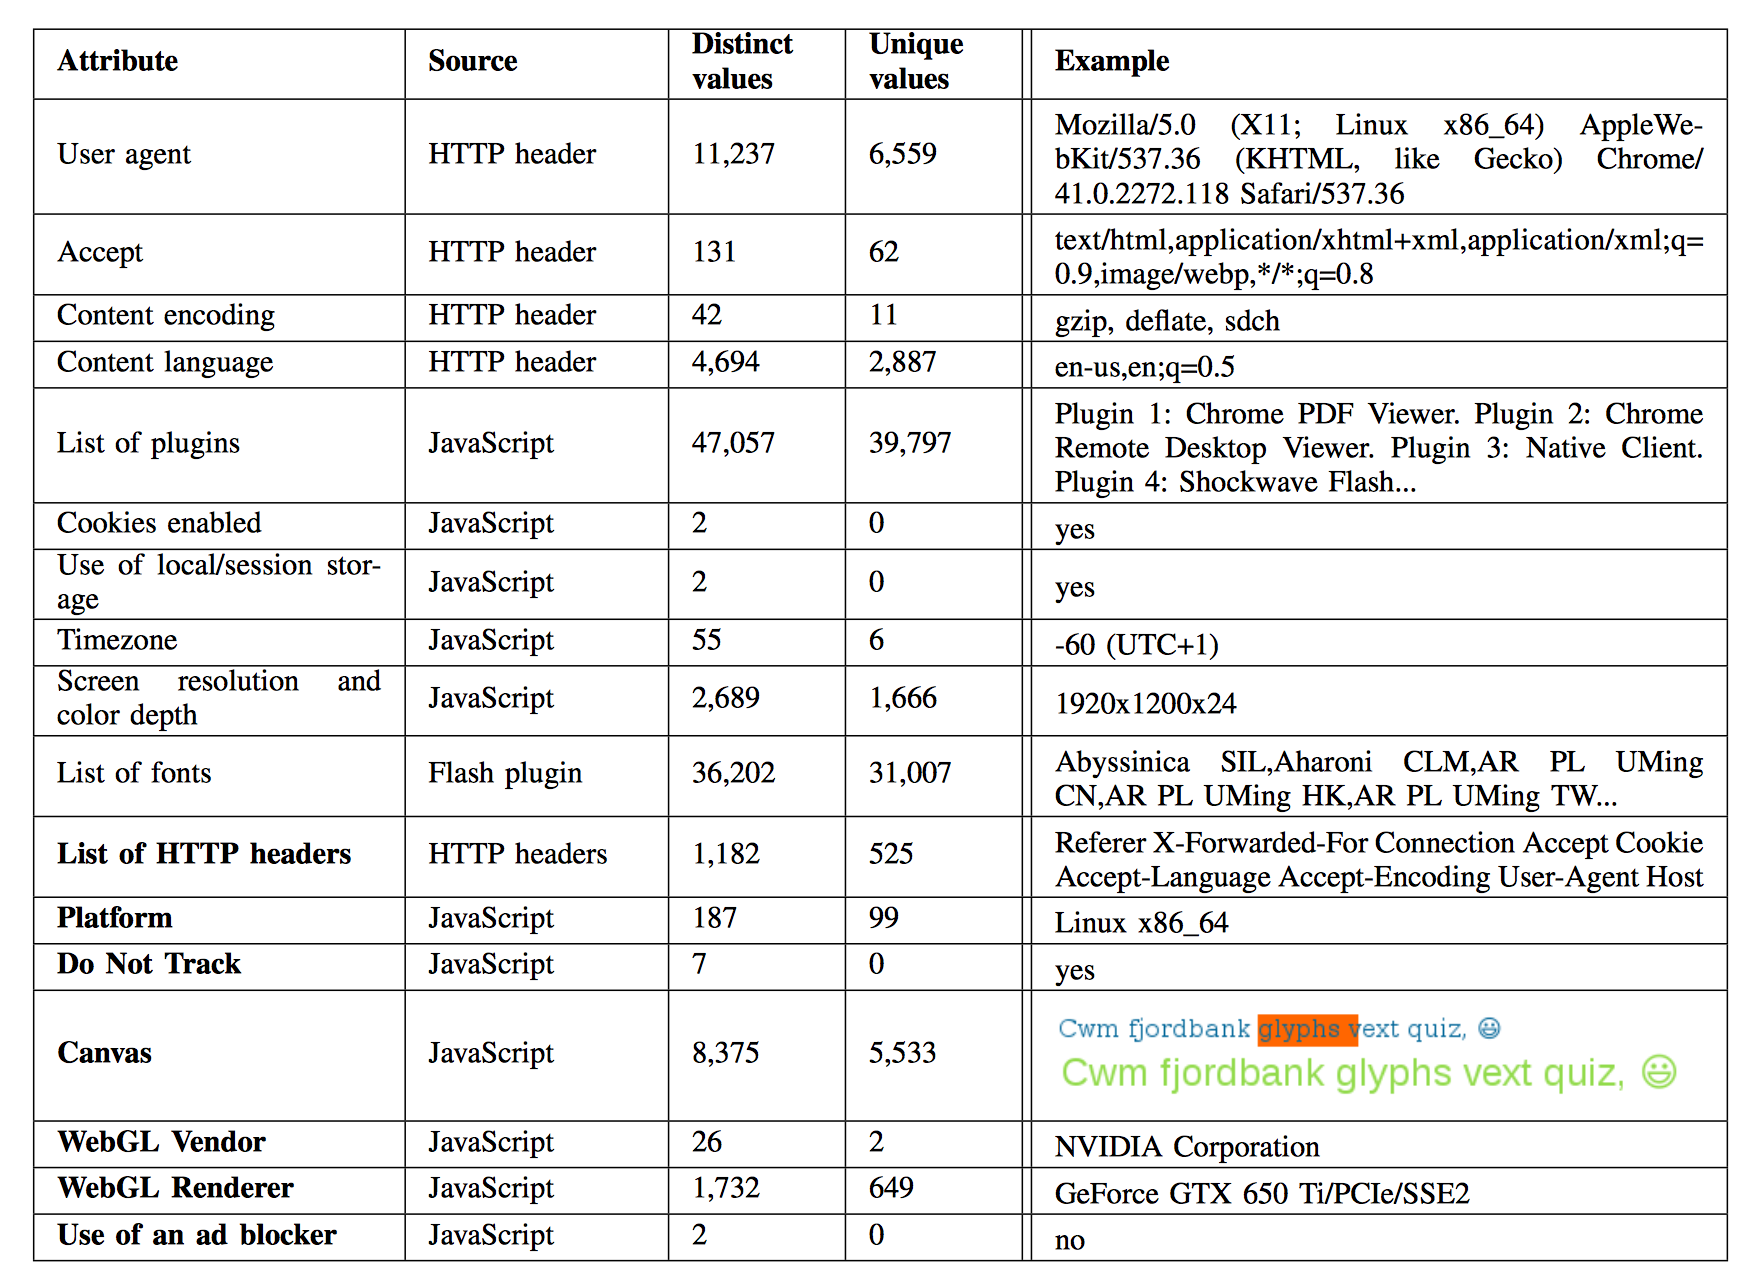
\includegraphics[width=\textwidth]{assets/amiunique.png}
    \caption{List of Attributes Fingerprinted for AmIUnique.org}
    \label{fig:amiunique}
\end{figure*}


According to Acar et al. \cite{acar:fpd}, browser fingerprinting technologies can be categorized by the approach they use to collect information: (1) JavaScript-based, (2) Plugin-based, (3) Extension-based, (4) Header-based and Server-side.
The rest of this section will go through in more detail about each of them.

\paragraph{JavaScript-Based Fingerprinting}
JavaScript is the default scripting language for almost all interactive web applications now. It provides functionality such as rendering of animation, submitting of user forms, and altering the content of the page dynamically. 
Other than the informative objects mentioned earlier (\verb|navigator| and \verb|screen|), JavaScript can also be used to identify users indirectly, such as obtaining browsing history or fine-grained timing information of the JavaScript engine at different browsers.

\paragraph{Plugin-Based Fingerprinting}
Plugins are equipped with capabilities to access the software and hardware properties of the underlying system. One of these common plugins is Flash that is used for displaying videos and games in the \verb|.swf| format. In order for the web pages to use Flash effectively, Flash exposes APIs to query information about the operating system, as well as the specific version of Flash installed.
Moreover, Flash also exposes APIs that allow one to list all the system fonts, which can vary from user to user. The difference in those fonts installed can again be used as an identifier for the user.
Therefore, the more plugins a user has installed, the more information can be exposed to fingerprinting software.

\paragraph{Extension-Based Fingerprinting}
A browser extension is a special software component that adds extra functionality to the browser, such as RSS reader or ad-blockers. Extensions are different from plugins as extensions provide additional functionality in the browser itself while plugins enable additional functionality for rendering a web page. Take one of the extensions that expose additional
information as an example: \verb|NoScript| \cite{noscript}, which is an extension that blocks executions of Web objects from any URL but those whitelisted. As explained by Mowery et al. \cite{mowery:fg}, one can prepare a list of URLs in the web page and see which of them are listed on the whitelist. The whitelist of the extension then can be used as an identifier to differentiate users from each other.

\paragraph{Header-Based and Server-Side}
This is one of the most basic fingerprinting techniques where the fingerprinters use information from the HTTP headers as identifiers. The HTTP headers contain information such as the IP address or Accept Headers in the request. Such information is readily available for all browsers and sent to  servers in the HTTP request.

Combining all these different practices together, the fingerprinter can obtain a large amount of information on a user.  Laperdrix et al. \cite{pierre:beauty} demonstrates that one can combine at least 17 attributes from various sources to create unique device fingerprints. As shown in Figure \ref{fig:amiunique}, the possible number of combinations of the different vlaues from those parameters is rather large, and the study successfully identified $81\%$ users out of 118,000 users.



\subsection{Fingerprinting for Authentication}
Despite the existing shortcomings of a password-based authentication methodology, it still remains the dominant method for web authentication. There are multiple ways to enhance the security of password-based authentication, such as the Multi-Factor Authentication model. Device fingerprinting can also be used to augment password-based authentication.
A number of commercial fraud detection services have already started using device fingerprinting in identifying fraudulent transactions.\cite{maxmind} \cite{parame} A user's device fingerprint is collected automatically and stored alongside their\ password.  The server can use a wide range of fingerprinting methods such as those described in earlier. The server can then verify the device fingerprint later during authentication.

The following sections will discuss the areas to consider when device fingerprinting is used to strengthen web authentication.


\subsubsection{Desired Properties}
In order to effectively augment user authentication with device fingerprinting, there are a number of properties that the device fingerprint should hold. A set of inappropriate fingerprinting practices may incur too many false negatives in the authentication process, denying legitimate users access or falling back to the most conservative authentication process too frequently. 
Compared to the general usage of fingeprinting in advertising, fingerprinting for authentication requires a higher level of accuracy in distinguishing users. A $80\%$ or $90\%$ accuracy is simply not enough. \cite{alca:dev}

In this section, we will be discussing the properties that make a set of fingerprinting practices a good augmentation for the authentication process:

\paragraph{Stablility across different scenarios}
It is normal for a user to have their device fingerprint change over time or in different scenarios. For example,  a user may be traveling across different time zones or switch between devices. 
A significant change in the device fingerprints will usually lead to a fallback on a less convenient but reliable authentication process, such as a one-time code sent to the user's phone or email. Therefore, using fingerprint practices that are reliable over time for a particular user is prefereable. Having more diverse metrics collected from different fingerprint practices will allow a small subset of values to vary without decreasing the overall stability of the fingerprint.

\paragraph{Repeatability on same device}
Repeatability is defined as the property whereby the same fingerprinting techniques generate the same results if the software, hardware, and network configuration of a device does not change. \cite{alca:dev}. It is related to but different from the stability requirement, which is primarily concerned  with changes in the device configuration.
For some  fingerprinting techniques, such as measuring the JavaScript rendering performance (determined and related to the underlying GPU/CPU performance and load at a specific instance), the same device may generate different results with other applications running: for example, trying to login when having a video compliation job running in the background might produce different fingerprints.

\paragraph {Resistence to spoofing}
An attacker can potentially spoof a device fingerprint by mimicking the properties or behaviour of the targeted device. Some fingerprinting techniques  have a low threshold for this kind of spoofing attack. For example, if the server relies on running a particular JavaScript script at the client side and retrieving the result from the client, then an attack can potentially replay the results to pretend to be the victim.
On the other hand, some fingerprint technique are more resistent to such spoofing, such as the IP address of the sources\cite{beverly:ip} or timestamps indicating clock skew from MAC protocol packets \cite{ara:wire}.

There are many other requirements that are not listed above in detail, such as the overhead in fingerprint collection, the convenience and level of action required from the user, and personalized identification information (the uniqueness of the fingerprints).


\subsubsection{Fingerprint Authentication Solution}
In this section, we discuss two strategies of using fingerprinting to augment authentication: (1) fingerprinting at session initialization, (2) fingerprinting throughout an authenticated session. 

\paragraph{Fingerprint at the start of session}
Fingerprint information is used as an additional authentication dimension alongside the normal password-based authentication (or other primary authentication method), and an authenticated session requires the matching of both the primary response as well as the fingerprint data stored.
In order for this strategy to work, the server must be able to store persistently the fingerprint data which is given by the user at registration. 
Such a strategy can be combined with two-factor authentication. For example, in the event where the device used for receiving SMS is stolen, a fingerprint of the stolen device might reveal the unusual state of it as the fingerprint check failed, which leads to additional security checks.

In general, this strategy can prevent or make the below attacks more difficult: 
\begin{itemize}
    \item \textbf{Naive Attack} A naive attack is defined as a conventional password-guessing attack that does not attempt to provide a matching fingerprint. A device fingerprint can effectively counter this attack since the attacker is assumed to launch the attack in a rather different environment. 
    \item \textbf{Optimized Password and Fingerprint Guessing}: The attacker might prepare common fingerprint profiles and use it along with to launch a naive password-guessing attack. A device fingerprint can effectively reduce the chances of success under this attack given that the fingeprint information expands the guessing space, and the attacker is only allowed a limited number of trials. 
    \item \textbf{Fingerprint Spoofing and Phishing}: Just like a normal password spoofing and phishing attack, the attacker can collect fingerprint information from users on top of the password. The level of spoofing resistence in the fingerprint used will then largely determine the feasibility of this attack. 
\end{itemize}

\paragraph{Fingerprint throughout an authenticated session}
In a typical password-based web authentication scheme, the server will return a cookie upon receiving a valid username and password so that the client will use the cookie as a proof of authentication in every request later on. This could be strenghened by validating the fingerprint information at each request. If the set of fingerprints that the server collects remains static, the recomputation of the fingerprint at each request is redundant.

A simple replay attack can be effecively prevented by hashing the fingerprint at the client with a counter before sending to the server, as demonstrated by \cite{preu:smart}. However, for a more powerful attack such as XSS attack, it is less effective. The attacker can launch a XSS targeted at the victim, and steal the plaintext device fingerprint and the counter at the client-side. Once obtaining the fingerprint plaintext, the attacker can reproduce the hash by incrementing the counter
and recomputing. In addition, such an attack is also possible even if the server dynamically changes the set of fignerprint attributes in each request \cite{unger:shpf} as the attacker can simply collect additional information about the target device once the hijacking is successful.



\section{Fingerprint Auth Plugin}
This section discusses the design and implementation of our device fingerprinting technique on a web application.
 
The aim of our project is to showcase the possibility that a unique device fingerprint could potentially replace passwords in scenarios where a user needs to be authenticated. In our web application, users are allowed to sign up an account using only an email. During registration, our web application will generate a unique fingerprint hash that pairs with the email provided. Once registered, users can proceed to login using their registered email - they will be authenticated based on the pair of information containing both email and fingerprint hash. This single-field input provides simplicity and ease for users, eliminating the need to remember passwords howbeit without compromising security. 

\subsection{Device Fingerprint Plugin}
The mechanism to generate a device fingerprint is the key and integral part of project. We built a plugin, consolidated into one single Javascript file that could analyze and collect a device’s information from a series of 27 components listed below. Each component is weighted according to its uniqueness across different devices. For instance, \textit{pixelRatio} is given a higher percentage than userAgent as it would vary more differently. The values and resulting percentages from each component is then combined into a hashed fingerprint unique for the device.

%%% TODO List of attributes
\begin{itemize}
    \item userAgent: the User-Agent string of the browser eg. \verb|Mozilla/5.0| (\verb|Windows NT 10.0|; \verb|Win64|)
    \item language: the current language used in the browser, eg. \verb|en-GB|
    \item colourDepth:  the colour depth of the device in bits eg. $24$.
      deviceMemory - the amount of memory on the device in gigabytes eg. $4$
  \item pixelRatio - ratio of device pixels to CSS pixels eg. \verb|2|
  \item hardwareConcurrency - number of logical processors eg. $8$
  \item screenResolution - width and height of the current screen eg. $864,1536$
  \item availableScreenResolution - width and height of the current screen available eg. $824,1536$
  \item  timezoneOffset - offset from the GMT timezone in minutes eg. $-480$
  \item timezone - current timezone eg. $Asia/Singapore$
  \item sessionStorage - whether the HTML5 session storage API is available eg. $true$
  \item localStorage - whether the HTML5 localStorage API is available eg. $true$
  \item indexedDb - whether the HTML5 indexedD API is available eg. $true$
  \item addBehavior - whether addBehaviour is available eg. $false$
  \item openDatabase - whether WebSQL is available eg. $true$
  \item cpuClass - CPU class of the device eg. \verb|Win32|
  \item platform - platform of the device eg. \verb|Win32|
  \item doNotTrack - whether the Do Not Track setting is on eg. $false$
  \item plugins - list of plugins installed
  \item canvas - canvas fingerprint of browser
  \item webgl - WebGL fingerprint of browser
  \item webglVendorAndRenderer - WebGL vendor and renderer of browser
  \item adBlock - whether the browser has an ad blocker installed eg. $false$
  \item touchSupport - whether the device has a touchscreen interface, with no. of touchpoints eg. $10, false,false$
  \item fonts - detection of all user installed fonts
  \item audio - audio fingerprint of device
\end{itemize}

The idea of a single-file Javascript plugin considers scalability whereby it could be imported into any web application for the purpose of generating a device’s fingerprint.

\subsection{Demo Web Application}
The plugin above has been fitted into our streamlined web application to exemplify the fingerprint-based authentication.

\begin{figure}[h]
    \centering
    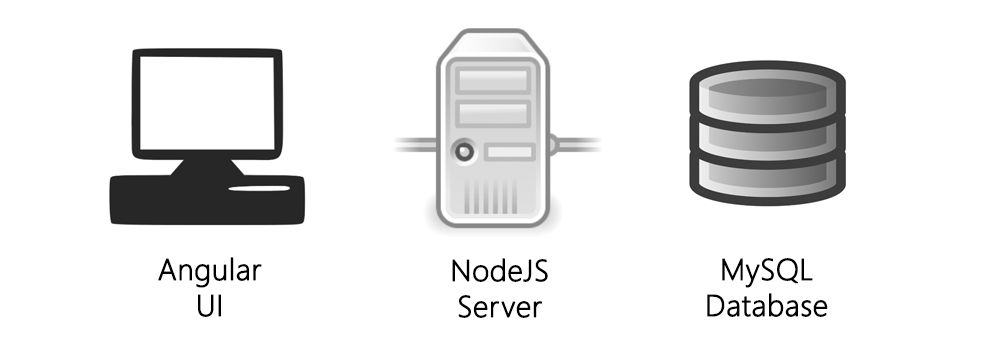
\includegraphics[width=0.5\textwidth]{assets/demo-flow.png}
    \caption{Demo Flow of Web Application}
    \label{fig:demo-flow}
\end{figure}

As shown in Figure \ref{fig:demo-flow}, our web application consists of three components - User Interface (UI), Server and a Database.

The front-end user interface that displays the registration and login page is built with Angular 6.0, designed with Material Design Bootstrap for aesthetics. The UI is in charged of calling the function of our fingerprint plugin to generate a device fingerprint and thereby package both user input email and hashed fingerprint into a JSON object, passing it to the NodeJS server.

The NodeJS server utilizes Express 4.0 API routing for communication of data between front-end and database. For storing and retrieving of data, it uses Flex.Query Processor Library to execute SQL statements to a MySQL instance.

\begin{itemize}
    \item \textbf{Sign Up Flow:}
        \begin{enumerate}
        \item User signs up with an email  
        \item UI generates fignerprint hash  
        \item UI sends fingerprint hash and email of the registering user to backend  
        \item UI displays the fingerprint hash to user  
        \item Backend stores fingerprint hash and email into the database  
        \end{enumerate}

    \item \textbf{Login Flow:}
        \begin{enumerate}
        \item User logs in with email  
        \item UI generates fingerprint hash  
        \item UI sends fingerprint hash and email to backend  
        \item Backend checks whether there exists any record for the pair of information and returns either true or false to authenticate the user  
        \item UI prompts login success / failure  
\end{enumerate}
\end{itemize}

\begin{figure}[h]
    \centering
    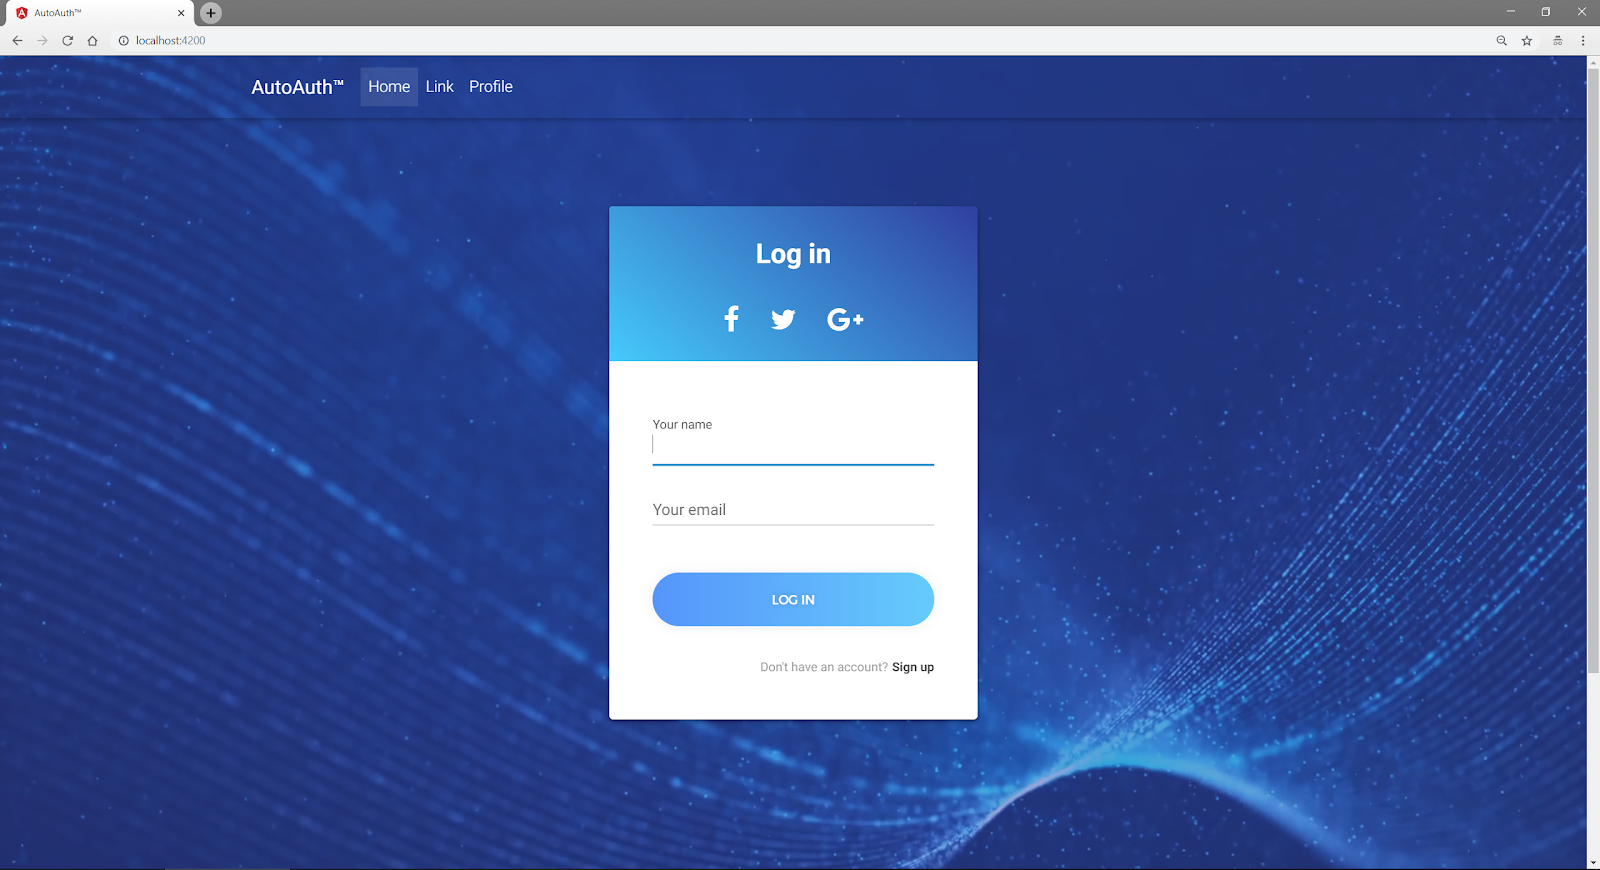
\includegraphics[width=0.5\textwidth]{assets/ui.png}
    \caption{UI for the Web Applicaiton}
    \label{fig:ui}
\end{figure}

\section{Extensions}
\subsection{Improvements to be made}
One of the issues regarding the current fingerprinting technology that we did not cover in depth is the comparison between accuracy and convenience of the technology. As mentioned previously in Section 3.3, in order to use fingerprinting technology as an authentication method, there needs to be stability across different scenarios. Minor changes made to a user's device such as a screen resolution change have to be handled either by accepting or rejecting the changes in the fingerprint. However, the only way that we can accept this change in our current implementation is by ignoring this specific set of data. This is because device fingerprinting results in a hash and any changes can cause the hash to be totally different.

\paragraph{Accuracy vs Convenience}
In order to increase the accuracy of fingerprinting technology, we have to include as many different data that can be acquired from the device as possible so as to get more unique values. This results in less convenience for the users as they have to fall back to a two factor authentication in order for the system to recompute their fingerprint. Further research will have to be conducted to find the set of data that is most optimized for both accuracy as well as convenience. Another method to improve the convenience without affecting too much of the accuracy is to use fuzzy hashing to compute the fingerprint hash as fuzzy hashing allows for small changes in the input without affecting the resulting hash. Therefore, it will then be able to handle changes that are small while still detecting large changes such as logging in from a completely different system.

\section{Conclusion}
In a nutshell, device fingerprinting is an effective and convenient method of device identification and we have examined the possibility of transforming this key idea into web-based user authentication using unique hashed fingerprints.

By combining various components of a device's properties, we could increase the fingerprint entropy as well as obtain a hash unqiue for an individual's device, correspondingly unique to an individual.

Although an device's fingerprint could change over time, we have considered that a user can be re-authenticated using a one-time password sent to their registered email.

It is worth noting that fingerprinting alone however, cannot prevent attacks such as session hijacking where a perpetrator can simply collect additional information about the target device once the hijacking is successful.

All in all, we think that fingerprinting is useful and provides a viable authentication method allowing users to be authenticated easily and such technology can be explored further in future security implementations.

% The following two commands are all you need in the
% initial runs of your .tex file to
% produce the bibliography for the citations in your paper.
\bibliographystyle{abbrv}
\bibliography{paper}  % sigproc.bib is the name of the Bibliography in this case
% You must have a proper ".bib" file
%  and remember to run:
% latex bibtex latex latex
% to resolve all references


%
% ACM needs 'a single self-contained file'!
% \subsection{Type Changes and {\subsecit Special} Characters}
% 
% \subsection{Math Equations}
% You may want to display math equations in three distinct styles:
% inline, numbered or non-numbered display.  Each of
% the three are discussed in the next sections.
% 
% \subsubsection{Inline (In-text) Equations}
% A formula that appears in the running text is called an
% inline or in-text formula.  It is produced by the
% \textbf{math} environment, which can be
% invoked with the usual \texttt{{\char'134}begin. . .{\char'134}end}
% construction or with the short form \texttt{\$. . .\$}. You
% can use any of the symbols and structures,
% from $\alpha$ to $\omega$, available in
% \LaTeX\cite{Lamport:LaTeX}; this section will simply show a
% few examples of in-text equations in context. Notice how
% this equation: \begin{math}\lim_{n\rightarrow \infty}x=0\end{math},
% set here in in-line math style, looks slightly different when
% set in display style.  (See next section).
% 
%


%
% \subsubsection{Display Equations}
% A numbered display equation -- one set off by vertical space
% from the text and centered horizontally -- is produced
% by the \textbf{equation} environment. An unnumbered display
% equation is produced by the \textbf{displaymath} environment.
% 
% Again, in either environment, you can use any of the symbols
% and structures available in \LaTeX; this section will just
% give a couple of examples of display equations in context.
% First, consider the equation, shown as an inline equation above:
% \begin{equation}\lim_{n\rightarrow \infty}x=0\end{equation}
% Notice how it is formatted somewhat differently in
% the \textbf{displaymath}
% environment.  Now, we'll enter an unnumbered equation:
% \begin{displaymath}\sum_{i=0}^{\infty} x + 1\end{displaymath}
% and follow it with another numbered equation:
% \begin{equation}\sum_{i=0}^{\infty}x_i=\int_{0}^{\pi+2} f\end{equation}
% just to demonstrate \LaTeX's able handling of numbering.
% 
% \subsection{Citations}
% Citations to articles \cite{bowman:reasoning, clark:pct, braams:babel, herlihy:methodology},
% conference
% proceedings \cite{clark:pct} or books \cite{salas:calculus, Lamport:LaTeX} listed
% in the Bibliography section of your
% article will occur throughout the text of your article.
% You should use BibTeX to automatically produce this bibliography;
% you simply need to insert one of several citation commands with
% a key of the item cited in the proper location in
% the \texttt{.tex} file \cite{Lamport:LaTeX}.
% The key is a short reference you invent to uniquely
% identify each work; in this sample document, the key is
% the first author's surname and a
% word from the title.  This identifying key is included
% with each item in the \texttt{.bib} file for your article.
% 
% The details of the construction of the \texttt{.bib} file
% are beyond the scope of this sample document, but more
% information can be found in the \textit{Author's Guide},
% and exhaustive details in the \textit{\LaTeX\ User's
% Guide}\cite{Lamport:LaTeX}.
% 
% This article shows only the plainest form
% of the citation command, using \texttt{{\char'134}cite}.
% This is what is stipulated in the SIGS style specifications.
% No other citation format is endorsed.
% 
% \subsection{Tables}
% Because tables cannot be split across pages, the best
% placement for them is typically the top of the page
% nearest their initial cite.  To
% ensure this proper ``floating'' placement of tables, use the
% environment \textbf{table} to enclose the table's contents and
% the table caption.  The contents of the table itself must go
% in the \textbf{tabular} environment, to
% be aligned properly in rows and columns, with the desired
% horizontal and vertical rules.  Again, detailed instructions
% on \textbf{tabular} material
% is found in the \textit{\LaTeX\ User's Guide}.
% 
% Immediately following this sentence is the point at which
% Table 1 is included in the input file; compare the
% placement of the table here with the table in the printed
% dvi output of this document.
% 
% \begin{table}
% \centering
% \caption{Frequency of Special Characters}
% \begin{tabular}{|c|c|l|} \hline
% Non-English or Math&Frequency&Comments\\ \hline
% \O & 1 in 1,000& For Swedish names\\ \hline
% $\pi$ & 1 in 5& Common in math\\ \hline
% \$ & 4 in 5 & Used in business\\ \hline
% $\Psi^2_1$ & 1 in 40,000& Unexplained usage\\
% \hline\end{tabular}
% \end{table}
% 
% To set a wider table, which takes up the whole width of
% the page's live area, use the environment
% \textbf{table*} to enclose the table's contents and
% the table caption.  As with a single-column table, this wide
% table will ``float" to a location deemed more desirable.
% Immediately following this sentence is the point at which
% Table 2 is included in the input file; again, it is
% instructive to compare the placement of the
% table here with the table in the printed dvi
% output of this document.
% 
% 
% \begin{table*}
% \centering
% \caption{Some Typical Commands}
% \begin{tabular}{|c|c|l|} \hline
% Command&A Number&Comments\\ \hline
% \texttt{{\char'134}alignauthor} & 100& Author alignment\\ \hline
% \texttt{{\char'134}numberofauthors}& 200& Author enumeration\\ \hline
% \texttt{{\char'134}table}& 300 & For tables\\ \hline
% \texttt{{\char'134}table*}& 400& For wider tables\\ \hline\end{tabular}
% \end{table*}
% % end the environment with {table*}, NOTE not {table}!
% 
% \subsection{Figures}
% Like tables, figures cannot be split across pages; the
% best placement for them
% is typically the top or the bottom of the page nearest
% their initial cite.  To ensure this proper ``floating'' placement
% of figures, use the environment
% \textbf{figure} to enclose the figure and its caption.
% 
% This sample document contains examples of \textbf{.eps}
% and \textbf{.ps} files to be displayable with \LaTeX.  More
% details on each of these is found in the \textit{Author's Guide}.
% 
% \begin{figure}
% \centering
% \epsfig{file=fly.eps}
% \caption{A sample black and white graphic (.eps format).}
% \end{figure}
% 
% \begin{figure}
% \centering
% \epsfig{file=fly.eps, height=1in, width=1in}
% \caption{A sample black and white graphic (.eps format)
% that has been resized with the \texttt{epsfig} command.}
% \end{figure}
% 
% 
% As was the case with tables, you may want a figure
% that spans two columns.  To do this, and still to
% ensure proper ``floating'' placement of tables, use the environment
% \textbf{figure*} to enclose the figure and its caption.
% 
% Note that either {\textbf{.ps}} or {\textbf{.eps}} formats are
% used; use
% the \texttt{{\char'134}epsfig} or \texttt{{\char'134}psfig}
% commands as appropriate for the different file types.
% 
% \subsection{Theorem-like Constructs}
% Other common constructs that may occur in your article are
% the forms for logical constructs like theorems, axioms,
% corollaries and proofs.  There are
% two forms, one produced by the
% command \texttt{{\char'134}newtheorem} and the
% other by the command \texttt{{\char'134}newdef}; perhaps
% the clearest and easiest way to distinguish them is
% to compare the two in the output of this sample document:
% 
% This uses the \textbf{theorem} environment, created by
% the\linebreak\texttt{{\char'134}newtheorem} command:
% \newtheorem{theorem}{Theorem}
% \begin{theorem}
% Let $f$ be continuous on $[a,b]$.  If $G$ is
% an antiderivative for $f$ on $[a,b]$, then
% \begin{displaymath}\int^b_af(t)dt = G(b) - G(a).\end{displaymath}
% \end{theorem}
% 
% The other uses the \textbf{definition} environment, created
% by the \texttt{{\char'134}newdef} command:
% \newdef{definition}{Definition}
% \begin{definition}
% If $z$ is irrational, then by $e^z$ we mean the
% unique number which has
% logarithm $z$: \begin{displaymath}{\log e^z = z}\end{displaymath}
% \end{definition}
% 
% \begin{figure}
% \centering
% \psfig{file=rosette.ps, height=1in, width=1in,}
% \caption{A sample black and white graphic (.ps format) that has
% been resized with the \texttt{psfig} command.}
% \end{figure}
% 
% Two lists of constructs that use one of these
% forms is given in the
% \textit{Author's  Guidelines}.
% 
% \begin{figure*}
% \centering
% \epsfig{file=flies.eps}
% \caption{A sample black and white graphic (.eps format)
% that needs to span two columns of text.}
% \end{figure*}
% and don't forget to end the environment with
% {figure*}, not {figure}!
%  
% There is one other similar construct environment, which is
% already set up
% for you; i.e. you must \textit{not} use
% a \texttt{{\char'134}newdef} command to
% create it: the \textbf{proof} environment.  Here
% is a example of its use:
% \begin{proof}
% Suppose on the contrary there exists a real number $L$ such that
% \begin{displaymath}
% \lim_{x\rightarrow\infty} \frac{f(x)}{g(x)} = L.
% \end{displaymath}
% Then
% \begin{displaymath}
% l=\lim_{x\rightarrow c} f(x)
% = \lim_{x\rightarrow c}
% \left[ g{x} \cdot \frac{f(x)}{g(x)} \right ]
% = \lim_{x\rightarrow c} g(x) \cdot \lim_{x\rightarrow c}
% \frac{f(x)}{g(x)} = 0\cdot L = 0,
% \end{displaymath}
% which contradicts our assumption that $l\neq 0$.
% \end{proof}
% 
% Complete rules about using these environments and using the
% two different creation commands are in the
% \textit{Author's Guide}; please consult it for more
% detailed instructions.  If you need to use another construct,
% not listed therein, which you want to have the same
% formatting as the Theorem
% or the Definition\cite{salas:calculus} shown above,
% use the \texttt{{\char'134}newtheorem} or the
% \texttt{{\char'134}newdef} command,
% respectively, to create it.
% 
% \subsection*{A {\secit Caveat} for the \TeX\ Expert}
% Because you have just been given permission to
% use the \texttt{{\char'134}newdef} command to create a
% new form, you might think you can
% use \TeX's \texttt{{\char'134}def} to create a
% new command: \textit{Please refrain from doing this!}
% Remember that your \LaTeX\ source code is primarily intended
% to create camera-ready copy, but may be converted
% to other forms -- e.g. HTML. If you inadvertently omit
% some or all of the \texttt{{\char'134}def}s recompilation will
% be, to say the least, problematic.
% 
% \section{Conclusions}
% This paragraph will end the body of this sample document.
% Remember that you might still have Acknowledgments or
% Appendices; brief samples of these
% follow.  There is still the Bibliography to deal with; and
% we will make a disclaimer about that here: with the exception
% of the reference to the \LaTeX\ book, the citations in
% this paper are to articles which have nothing to
% do with the present subject and are used as
% examples only.
% %\end{document}  % This is where a 'short' article might terminate
% 
% %ACKNOWLEDGMENTS are optional
% \section{Acknowledgments}
% This section is optional; it is a location for you
% to acknowledge grants, funding, editing assistance and
% what have you.  In the present case, for example, the
% authors would like to thank Gerald Murray of ACM for
% his help in codifying this \textit{Author's Guide}
% and the \textbf{.cls} and \textbf{.tex} files that it describes.

% %APPENDICES are optional
% %\balancecolumns
% \appendix
% %Appendix A
% \section{Headings in Appendices}
% The rules about hierarchical headings discussed above for
% the body of the article are different in the appendices.
% In the \textbf{appendix} environment, the command
% \textbf{section} is used to
% indicate the start of each Appendix, with alphabetic order
% designation (i.e. the first is A, the second B, etc.) and
% a title (if you include one).  So, if you need
% hierarchical structure
% \textit{within} an Appendix, start with \textbf{subsection} as the
% highest level. Here is an outline of the body of this
% document in Appendix-appropriate form:
% \subsection{Introduction}
% \subsection{The Body of the Paper}
% \subsubsection{Type Changes and  Special Characters}
% \subsubsection{Math Equations}
% \paragraph{Inline (In-text) Equations}
% \paragraph{Display Equations}
% \subsubsection{Citations}
% \subsubsection{Tables}
% \subsubsection{Figures}
% \subsubsection{Theorem-like Constructs}
% \subsubsection*{A Caveat for the \TeX\ Expert}
% \subsection{Conclusions}
% \subsection{Acknowledgments}
% \subsection{Additional Authors}
% This section is inserted by \LaTeX; you do not insert it.
% You just add the names and information in the
% \texttt{{\char'134}additionalauthors} command at the start
% of the document.
% \subsection{References}
% Generated by bibtex from your ~.bib file.  Run latex,
% then bibtex, then latex twice (to resolve references)
% to create the ~.bbl file.  Insert that ~.bbl file into
% the .tex source file and comment out
% the command \texttt{{\char'134}thebibliography}.
% This next section command marks the start of
% Appendix B, and does not continue the present hierarchy
% \section{More Help for the Hardy}
% The acm\_proc\_article-sp document class file itself is chock-full of succinct
% and helpful comments.  If you consider yourself a moderately
% experienced to expert user of \LaTeX, you may find reading
% it useful but please remember not to change it.
% \balancecolumns
% % That's all folks!
\end{document}
